% =====================================================================
%  IEEE conference paper
%  Compile:  pdflatex main.tex   (run twice so cross-references settle)
%  Figures expected in ./figures/
% =====================================================================
\documentclass[conference,a4paper]{IEEEtran}
\IEEEoverridecommandlockouts

\usepackage{cite}
\usepackage{amsmath,amssymb,amsfonts}
\usepackage{algorithm}
\usepackage{algorithmic}
\usepackage{graphicx}
% Figures live in <repo>/figures/. This resolves whether the file is
% compiled from paper/ or from the repository root.
\graphicspath{{../}{./}}
\usepackage{textcomp}
\usepackage{booktabs}
\usepackage{array}
\usepackage{multirow}
\usepackage{url}
\usepackage[hidelinks]{hyperref}

\newcommand{\hlt}[1]{\textbf{#1}}

\begin{document}

\title{What Survives a Strict Split? An Empirical Audit of
       Long-Document Screenplay Modelling for IMDb Rating Prediction}

\author{
\IEEEauthorblockN{1\textsuperscript{st} Given Name Surname}
\IEEEauthorblockA{\textit{dept.\ name of organization} \\
\textit{name of organization}\\
City, Country \\
email@address}
\and
\IEEEauthorblockN{2\textsuperscript{nd} Given Name Surname}
\IEEEauthorblockA{\textit{dept.\ name of organization} \\
\textit{name of organization}\\
City, Country \\
email@address}
\and
\IEEEauthorblockN{3\textsuperscript{rd} Given Name Surname}
\IEEEauthorblockA{\textit{dept.\ name of organization} \\
\textit{name of organization}\\
City, Country \\
email@address}
}

\maketitle

% =====================================================================
\begin{abstract}
Screenplay-to-rating regression is usually reported on a random split of
an archival corpus. We argue that this number is not the number a reader
wants, and we measure the gap. Working from a corpus of $5{,}204$
IMSDb screenplays joined to IMDb metadata, we first run a record-identity
audit --- content SHA-256 digests, IMDb identifiers, title$\times$year
keys, and a normalised title-family key --- and publish the resulting
exclusion ledger, which retains $5{,}164$ records after removing nine
sub-1\,KB fragments, four corrupt release years, and twenty-seven records
whose positional identity in the archived embedding matrix cannot be
resolved uniquely. We then quantify a defect that is invisible at the API
surface: the pipeline slides a $256$-\emph{word} window over each script,
but the encoder admits only $254$ WordPiece \emph{tokens}, so
$98.45\%$ of windows are cut and $31.60\%$ of all tokens never reach the
model. Finally we evaluate identical representations and learners under
three partitions --- random $k$-fold, title-family \textsc{GroupKFold},
and a chronological 2020--2025 holdout. Skill is strongly
protocol-dependent: the best system reports $R^{2}=0.549$
$[0.530, 0.567]$ under random folds, $0.536$ $[0.516, 0.554]$ once
franchises are held together, and $0.309$ $[0.199, 0.404]$ when the test
set lies in the future. Block-permutation analysis on the temporal
holdout explains why. Release year and decade, which jointly supply
$36.6\%$ of in-sample split gain, contribute exactly
$\Delta\mathrm{MAE}=0.000$ once the test years fall outside the training
range, while runtime alone ($+0.199$) matches the entire $384$-dimensional
sentence-embedding block ($+0.195$). Semantic embeddings survive the
strict split; the calendar confound does not.
\end{abstract}

\begin{IEEEkeywords}
data leakage, evaluation protocol, sentence embeddings, long-document
NLP, screenplay analysis, temporal generalisation, grouped
cross-validation.
\end{IEEEkeywords}

% =====================================================================
\section{Introduction}

A feature-film screenplay runs to roughly $25{,}000$ words. Sentence
encoders read $256$ tokens. That mismatch is the central engineering
problem in screenplay modelling, and the usual answer --- slide a window,
embed each window, average the results --- is cheap, reproducible, and
widely used. What is far less often examined is whether the evaluation
wrapped around that pipeline measures anything a practitioner could rely
on, because an archival screenplay corpus assembled from a community
repository carries two structural hazards that a shuffled train/test
split will silently convert into apparent skill.

The first hazard is duplication. Community archives accumulate the same
work under several file names, franchises share vocabulary and structure
across installments, and remakes reuse plot and dialogue wholesale. Under
a random partition, a near-copy in the training set makes its twin in the
test set trivially predictable. The effect is not exotic; it is the
dominant failure mode catalogued in surveys of leakage-driven
irreproducibility across applied machine learning~\cite{kapoor2023}, and
it has been documented specifically for train--test overlap in NLP
benchmarks~\cite{lewis2021,elangovan2021}.

The second hazard is time. Ratings in an archival corpus are collected
once, at scrape time, but the films span a century, and both the
selection process and the rating behaviour of the audience drift. A model
given a release-year feature can recover a large share of target variance
from the calendar alone, without reading a single line of dialogue. That
shortcut evaporates the moment the test films are drawn from years the
model never saw, which is the only setting in which a screenplay-stage
predictor would actually be deployed.

Layered underneath both is a quieter defect specific to chunked
long-document pipelines. Chunking is almost always specified in words;
truncation always happens in subword tokens. Nobody is told when the
budget is exceeded --- the encoder simply drops the tail --- so a
configuration that reads as ``$256$-word windows with $50$-word overlap''
can in practice discard a third of the corpus without emitting a single
warning.

This paper is an audit, not a leaderboard entry. We take an existing
SBERT-plus-gradient-boosting pipeline over $5{,}204$ IMSDb screenplays and
ask what its reported performance is actually made of. Three
contributions follow.

\begin{itemize}
\item \hlt{C1 --- A record-identity protocol and its exclusion ledger.}
  We define film identity through four keys --- content SHA-256 digest,
  IMDb identifier, title$\times$year, and a normalised title-family stem
  --- audit all $5{,}204$ joined records against each, and report every
  exclusion (Section~\ref{sec:corpus}). The audited corpus contains no
  duplicate identifiers and no duplicate title$\times$year pairs, but
  $80$ title collisions and $164$ multi-member title families that a
  random split would happily straddle.
\item \hlt{C2 --- A measurement of silent truncation.} Running the
  encoder's own tokeniser over the pipeline's own windows, we find that
  $98.45\%$ of $256$-word windows exceed the $254$-token content budget
  and that $31.60\%$ of WordPiece tokens are discarded before the encoder
  sees them, with a median window of $371$ tokens against a budget of
  $254$ (Section~\ref{sec:tokens}).
\item \hlt{C3 --- A three-protocol evaluation with paired inference.}
  Holding representation and learner fixed, we vary only the partition:
  random $k$-fold, title-family \textsc{GroupKFold}, and a chronological
  2020--2025 holdout. We report bootstrap intervals, paired Wilcoxon
  signed-rank tests with matched-pairs effect sizes, and a
  block-permutation attribution that isolates which feature families
  survive temporal extrapolation (Sections~\ref{sec:results}
  and~\ref{sec:xai}).
\end{itemize}

We do not claim a new state of the art. We claim that the difference
between $R^{2}=0.549$ and $R^{2}=0.309$ on the same corpus, the same
features, and the same learner is the finding.

% =====================================================================
\section{Related Work}

\subsection{Computational analysis of screenplays}

Early work treated the script as a feature source for commercial
forecasting. Eliashberg et al.~\cite{ref3} extracted genre, content, and
semantic descriptors from spec scripts and fed a kernel regression to
predict return on investment; Hunter et al.~\cite{ref4} pushed a similar
text-analytic pipeline toward box-office revenue. Both established the
premise this paper inherits --- that a screenplay carries measurable
signal about reception --- and both evaluated on randomly partitioned
archival collections.

A second strand reads narrative structure rather than commercial
outcome. Reagan et al.~\cite{ref5} recovered six recurring emotional arc
shapes from sentiment trajectories; Ramakrishna et al.~\cite{ref6}
quantified linguistic differences in character portrayal; Chu et
al.~\cite{ref12} added audiovisual channels. Downstream classification
tasks built on script text include MPAA age-suitability
rating~\cite{ref10,ref34}, severity prediction~\cite{ref11}, and tag
assignment from plot synopses~\cite{ref35}. Screenplay quality assessment
in the awards-nomination framing~\cite{ref38} is the closest analogue to
rating regression, and it shares our target's central difficulty: the
label is an aggregate social judgement, only partly a function of the
text.

\subsection{Box-office and rating forecasting}

Outside the script itself, forecasting has drawn on production
metadata~\cite{ref15}, social-media volume~\cite{ref21,ref23}, Twitter
signals~\cite{ref22}, Wikipedia activity~\cite{ref24}, trailer
content~\cite{ref16}, and review sentiment~\cite{ref18,ref28}. IMDb
rating regression from tabular and textual metadata is by now a standard
applied exercise~\cite{ref17,ref26,ref29}, with deep-learning variants for
serial content~\cite{ref27} and multi-task formulations that fold
sentiment and diffusion together~\cite{ref30}. The reported figures span
a wide range, and the partitions behind them are rarely specified beyond
a random seed. Vogel's industry account~\cite{ref25} is a useful
corrective on the ceiling: theatrical outcomes are dominated by release
strategy, competition, and marketing spend, none of which is legible in
the script.

\subsection{Representations for long documents}

Sentence-BERT~\cite{ref2} produces dense sentence-level embeddings from a
Siamese objective and is the encoder we audit. Its native context is
short, so document-level use requires either hierarchical
attention~\cite{ref19}, sparse attention over longer
sequences~\cite{ref1}, or chunk-and-pool aggregation. Chunk-and-pool is
the pragmatic default: it needs no fine-tuning, runs on CPU, and scales
linearly. Its cost is that the aggregation function is fixed rather than
learned, and --- as we measure in Section~\ref{sec:tokens} --- that the
chunk boundary is usually specified in a unit the encoder does not use.
Classical $n$-gram TF-IDF remains a competitive lexical control on long
technical text and is included here for exactly that reason.

\subsection{Leakage and split design in archival NLP}

The methodological literature we lean on is not about films. Gorman and
Bedrick~\cite{gorman2019} showed that system rankings in POS tagging
reorder under alternative random splits; S{\o}gaard et
al.~\cite{sogaard2021} generalised the argument and recommended split
designs that stress the generalisation actually claimed. Lewis et
al.~\cite{lewis2021} found that a large fraction of open-domain QA test
questions have near-duplicates in training, and Elangovan et
al.~\cite{elangovan2021} formalised train--test overlap measurement.
Kapoor and Narayanan~\cite{kapoor2023} catalogue leakage taxonomies
across disciplines and argue for pre-registration of the split.
Temporal generalisation has its own line~\cite{lazaridou2021}, as does
documentation of corpus provenance~\cite{bender2018,dodge2021}. Applying
these instruments to a screenplay corpus is, to our knowledge, new; the
findings in Section~\ref{sec:results} suggest the exercise was overdue.

% =====================================================================
\section{Corpus Integrity and Exclusion Audit}
\label{sec:corpus}

\subsection{Source and join}

The corpus joins full screenplay texts scraped from the Internet Movie
Script Database (IMSDb) to IMDb metadata on a per-film basis. Each of the
$5{,}204$ joined records carries a title, release year, decade bin, IMDb
identifier, runtime in minutes, an IMDb rating on the $1.0$--$10.0$ scale
at one-decimal resolution, and a path to the script file. Ratings have
mean $5.98$, median $5.80$, and standard deviation $1.44$; runtimes span
$45$--$254$ minutes with median $99$.

\subsection{Four identity keys}

Deduplication is only as good as the notion of identity behind it, so we
audit four keys of decreasing strictness.

\emph{Content digest.} For a script file with byte content $b$, the key
is $\mathrm{SHA256}(b)$, rendered as a $64$-character hexadecimal
digest. Two records collide if and only if their files are
byte-identical, which catches the re-upload-under-a-new-name case that no
metadata key can see. Collisions are resolved by retaining the earliest
record in load order and discarding the rest.

\emph{IMDb identifier.} The \texttt{tt}-prefixed identifier is the
canonical film key and catches the case where the same film was collected
twice with different file names and slightly different titles.

\emph{Title$\times$year.} A fallback for records whose identifier is
missing or malformed.

\emph{Title family.} The loosest key, and the one that matters for split
design. We normalise a title $t$ by case-folding, stripping
non-alphanumeric characters, removing a leading article, and iteratively
deleting a trailing sequel marker --- an Arabic numeral, a Roman numeral
up to $\mathrm{X}$, or a \texttt{part}~$n$ construction. \emph{Toy
Story}, \emph{Toy Story 2} and \emph{Toy Story 3} therefore map to the
single family \texttt{toy story}. Families are not deduplicated; they are
the grouping variable for Section~\ref{sec:splits}. Algorithm~\ref{alg:fam}
states the normalisation precisely; the trailing-marker deletion is
applied to a fixed point, so \emph{Rocky II} and \emph{Rocky Part 2}
collapse to the same stem.

\begin{algorithm}[t]
\caption{Title-family key $\varphi(t)$}
\label{alg:fam}
\begin{algorithmic}[1]
\REQUIRE raw title string $t$
\ENSURE family stem used as the grouping variable
\STATE $u \leftarrow \textsc{Lowercase}(\textsc{Trim}(t))$
\STATE $u \leftarrow \textsc{Replace}(u,\ \texttt{[\^{}a-z0-9\textbackslash s]},\ \text{`` ''})$
  \COMMENT{drop punctuation}
\STATE $u \leftarrow \textsc{CollapseSpaces}(u)$
\STATE $u \leftarrow \textsc{StripPrefix}(u,\ \{\texttt{the},\texttt{a},\texttt{an}\})$
\REPEAT
  \STATE $u_{\text{prev}} \leftarrow u$
  \STATE $u \leftarrow \textsc{StripSuffix}\bigl(u,\ (\texttt{part}\ )?\,
         (\,d^{+} \mid \textsc{Roman}_{1..10}\,)\bigr)$
\UNTIL{$u = u_{\text{prev}}$}
\RETURN $u \neq \varepsilon\ ?\ u : \textsc{Lowercase}(\textsc{Trim}(t))$
\end{algorithmic}
\end{algorithm}

\subsection{The exclusion flow}
\label{sec:flow}

Let $\mathcal{R}_0$ be the joined record set, $|\mathcal{R}_0| = 5{,}204$.
The pipeline is a composition of four filters applied in a fixed order,
each defined by a predicate on a record $r$:
\begin{align}
\pi_{\text{len}}(r)  &\equiv |\mathrm{text}(r)| \ge 1000 \ \text{characters},\\
\pi_{\text{hash}}(r) &\equiv \mathrm{SHA256}\bigl(\mathrm{bytes}(r)\bigr)
   \notin \mathcal{H}_{<r},\\
\pi_{\text{year}}(r) &\equiv \mathrm{yr}(r) \in [1900,\, 2025],\\
\pi_{\text{id}}(r)   &\equiv \text{positional identity of } r
   \text{ is unique},
\end{align}
where $\mathcal{H}_{<r}$ is the set of digests already seen in load order,
so $\pi_{\text{hash}}$ retains exactly one representative per digest. The
surviving sets are nested,
\begin{equation}
\label{eq:flow}
\mathcal{R}_4 \subseteq \mathcal{R}_3 \subseteq \mathcal{R}_2
\subseteq \mathcal{R}_1 \subseteq \mathcal{R}_0 ,
\qquad
\mathcal{R}_{k} = \{\, r \in \mathcal{R}_{k-1} : \pi_k(r) \,\},
\end{equation}
and the realised cardinality chain on this corpus is
\begin{equation}
\label{eq:chain}
5{,}204
\;\xrightarrow{\ \pi_{\text{len}}\ } 5{,}195
\;\xrightarrow{\ \pi_{\text{hash}}\ } 5{,}195
\;\xrightarrow{\ \pi_{\text{year}}\ } 5{,}191
\;\xrightarrow{\ \pi_{\text{id}}\ } 5{,}164 .
\end{equation}

The second arrow is the one to read carefully. It is an identity map
\emph{on the subset over which the digest could be evaluated}
(Section~\ref{sec:hashscope}), not a corpus-wide null result: content
hashing requires the raw text, and $356$ of the $5{,}204$ files are
distributed with the code. Over those $356$ the digest audit returns zero
collisions. The metadata identity keys, which are computable for all
$5{,}204$ records, likewise return zero duplicate IMDb identifiers and
zero duplicate title$\times$year pairs, which bounds --- without
eliminating --- the residual duplication that a full-corpus pass could
still uncover. Should such a pass find $m$ collisions, only the second
arrow in \eqref{eq:chain} changes, and every downstream count shifts by
$m$; the protocol itself is unaffected.

\subsection{Audit results}

Table~\ref{tab:audit} is the full ledger for the flow of
Section~\ref{sec:flow}, and the nesting in \eqref{eq:flow} means every
row of it is a strict subset of the row above. Three observations deserve
comment.

\begin{table}[t]
\caption{Corpus integrity audit and exclusion ledger. Percentages are of
the $5{,}204$ joined records.}
\label{tab:audit}
\centering
\small
\begin{tabular}{lrr}
\toprule
\textbf{Check / exclusion} & \textbf{Count} & \textbf{\%} \\
\midrule
Joined records (IMSDb $\bowtie$ IMDb)      & 5{,}204 & 100.00 \\
\addlinespace[2pt]
\multicolumn{3}{l}{\emph{Identity keys}}\\
Distinct script file names                 & 5{,}204 & 100.00 \\
Distinct IMDb identifiers                  & 5{,}204 & 100.00 \\
Duplicate title$\times$year pairs          &       0 &   0.00 \\
Title collisions (same title, other year)  &  80 groups / 165 rec. & 3.17 \\
SHA-256 duplicate digests (audited subset) &       0 & --- \\
\addlinespace[2pt]
\multicolumn{3}{l}{\emph{Exclusions}}\\
Script text $<1{,}000$ characters          &       9 &   0.17 \\
Release year outside $[1900, 2025]$        &       4 &   0.08 \\
Unresolvable positional identity           &      27 &   0.52 \\
\midrule
\textbf{Analysis corpus}                   & \textbf{5{,}164} & \textbf{99.23} \\
\addlinespace[2pt]
Title families                             & 4{,}979 & --- \\
\quad multi-member families                &     164 & --- \\
\quad largest family                       &       4 & --- \\
\bottomrule
\end{tabular}
\end{table}

\emph{No exact film duplicates at the metadata level.} All $5{,}204$
identifiers are distinct and no title$\times$year pair repeats. This is a
genuinely clean join, and it means the leakage channel in this corpus is
not naive record duplication.

\emph{Eighty title collisions, all legitimate.} Eighty titles appear more
than once, spanning $165$ records, but every collision pairs distinct
identifiers and distinct years --- these are remakes and same-title
unrelated films, not duplicates. We retain them and place them in a
shared family, because a remake shares premise, character names, and
often substantial dialogue with its predecessor. Grouping is the correct
treatment; deletion would discard real data.

\emph{Metadata corruption is present and reaches the model.} Four records
carry release years of $1080$ or $1088$, transparently mis-typed $1980$
and $1988$ (\emph{Breaker Morant}, \emph{Mississippi Burning},
\emph{Torch Song Trilogy}, \emph{The Blues Brothers}). We drop them
rather than silently repair them. The derived decade column is worse: the
label encoder fitted by the shipped pipeline holds $14$ distinct decade
strings, among them \texttt{1080s}, \texttt{1900s} and \texttt{1996s},
and it encodes them as an \emph{ordinal} integer. Three corrupt levels
therefore enter the feature matrix as legitimate ordinal positions.
Section~\ref{sec:xai} shows that this feature contributes essentially
nothing, which is fortunate rather than by design.

Twenty-seven further records are excluded for a reproducibility reason
rather than a data-quality one. The archived embedding matrix stores rows
in loader order without a record key, and the loader had already dropped
nine sub-1\,KB scripts, so row $i$ of the matrix is not record $i$ of the
spreadsheet. We reconstruct the offset function from the committed split
bookkeeping --- $780$ test records anchor it exactly through their file
names, $779$ validation records constrain it further through
title-and-rating agreement --- and recover a mapping consistent with all
$1{,}559$ anchors. Twenty-seven positions inside the reconstruction gaps
admit more than one consistent assignment; we drop them rather than
guess. This is a self-inflicted wound of the original pipeline, and it is
the concrete argument for storing an immutable record key alongside any
cached representation.

\subsection{Scope of the content-digest pass}
\label{sec:hashscope}

One qualification must be stated plainly, because it bounds C1. The
SHA-256 pass requires the raw text, and the script corpus is not
redistributed with the code repository; $356$ of the $5{,}204$ files are
available in the public snapshot. Over those $356$ files the digest audit
returns zero duplicate groups. The metadata keys above --- identifier,
title$\times$year, and family --- are computed over all $5{,}204$
records and are unaffected. A full-corpus digest pass is a one-command
operation once the text is restored, and the audit code is released with
the paper; until then, our exact-duplicate claim is verified on the
distributed subset and asserted only there.

% =====================================================================
\section{Methodology and Representations}
\label{sec:method}

\subsection{Structural screenplay statistics}

Sixteen statistics are computed from the raw, uncleaned script text.
Table~\ref{tab:vardef} defines all nineteen numeric predictors --- the
sixteen structural statistics plus the three metadata columns --- with
corpus-level scale and split gain. Six are size
measures (\texttt{char\_count}, \texttt{word\_count},
\texttt{line\_count}, \texttt{sentence\_count}, \texttt{scene\_count},
\texttt{words\_per\_scene}); three describe lexical sophistication
(\texttt{avg\_word\_length}, \texttt{unique\_word\_ratio},
\texttt{long\_word\_ratio}, the last being the share of tokens of eight
or more characters); two describe sentence geometry
(\texttt{avg\_sentence\_length}, \texttt{sentence\_length\_std}); two
describe dialogue (\texttt{dialogue\_density}, the share of lines that
match an ALL-CAPS speaker-cue pattern, and
\texttt{unique\_characters}); two are emotional proxies
(\texttt{exclamation\_ratio}, \texttt{question\_ratio}, both per hundred
words); and one is a stage-direction proxy (\texttt{action\_density},
bracketed and parenthesised spans per hundred words). Scene count is the
number of case-insensitive \texttt{INT.}/\texttt{EXT.} matches, so
\texttt{words\_per\_scene} is an inverse tempo measure --- larger values
mean longer scenes and slower cutting. All sixteen are computed on the
\emph{raw} file, before either cleaning pass, so they describe the
transcript as archived rather than the text the encoder receives.

Two of the sixteen are close to degenerate on this corpus, and the audit
makes it visible before any model is fitted. Mean
\texttt{dialogue\_density} is $0.0087$ with standard deviation $0.0361$,
and mean \texttt{unique\_characters} is $3.41$. A feature film does not
have three speaking parts. The speaker-cue regular expression assumes a
\texttt{NAME:} convention that most IMSDb transcripts do not follow, so
both features encode transcription format rather than dramaturgy.
\texttt{scene\_count} has the same character: mean $19.0$ against a
standard deviation of $54.5$.

\subsection{Token-aligned chunking and mean pooling}
\label{sec:tokens}

Let a screenplay be a word sequence $D = (w_1, \dots, w_N)$ obtained by
whitespace splitting after light normalisation that removes bracketed
stage directions, ALL-CAPS speaker cues, \texttt{INT.}/\texttt{EXT.}
markers, and timestamps while preserving case and sentence punctuation.
With window length $L = 256$ and overlap $o = 50$, the stride is
\begin{equation}
s \;=\; L - o \;=\; 206 ,
\end{equation}
and the $j$-th window is
\begin{equation}
C_j \;=\; \bigl(w_{(j-1)s+1}, \dots, w_{\min\{(j-1)s+L,\; N\}}\bigr),
\end{equation}
for $j = 1, \dots, M$ with
\begin{equation}
M \;=\;
\begin{cases}
1, & N \le L,\\[2pt]
\left\lceil \dfrac{N - L}{s} \right\rceil + 1, & N > L .
\end{cases}
\end{equation}
Each window is encoded by $f: \mathcal{C} \to \mathbb{R}^{d}$ with
$d = 384$, and the document representation is the arithmetic mean
\begin{equation}
\label{eq:meanpool}
e(D) \;=\; \frac{1}{M} \sum_{j=1}^{M} f(C_j) .
\end{equation}

Equation~\eqref{eq:meanpool} has a property worth stating, because the
encoder L2-normalises its output: every $f(C_j)$ lies on the unit sphere,
so
\begin{equation}
\label{eq:norm}
\bigl\| e(D) \bigr\|_2^2
= \frac{1}{M^2}\Bigl( M + 2\!\!\sum_{1 \le i < j \le M}\!\!
  \langle f(C_i), f(C_j)\rangle \Bigr),
\end{equation}
which equals $1$ only when all windows embed identically and falls toward
$1/\sqrt{M}$ as they decorrelate. The norm of a mean-pooled screenplay
embedding is therefore a coherence statistic, and averaging over $M$
windows shrinks any single window's influence by $1/M$. With a median of
$36$ windows per script, no scene survives pooling as a distinguishable
signal.

\hlt{The word/token mismatch.} The encoder's transformer accepts
$T_{\max} = 256$ positions, two of which are consumed by \texttt{[CLS]}
and \texttt{[SEP]}. The content budget is therefore
\begin{equation}
B \;=\; T_{\max} - 2 \;=\; 254
\end{equation}
WordPiece tokens, while $C_j$ is defined by a count of $256$
\emph{words}. Writing $\tau(\cdot)$ for the tokeniser, the encoder in
fact sees $\tau(C_j)$ truncated to its first $B$ entries, and the
discarded fraction for a document is
\begin{equation}
\rho(D) \;=\; 1 - \frac{\sum_{j=1}^{M} \min\bigl\{|\tau(C_j)|,\, B\bigr\}}
                        {\sum_{j=1}^{M} |\tau(C_j)|} .
\end{equation}

Running the encoder's own tokeniser over the pipeline's own windows on
the $356$ available scripts yields $14{,}558$ windows with median length
$371$ tokens, mean $369.3$, $90$th percentile $405$, $99$th percentile
$453$, and maximum $613$ (Fig.~\ref{fig:tokens}). The consequences:
$98.45\%$ of windows exceed $B$, and $\rho$ evaluated corpus-wide is
$0.3160$, with a per-script mean of $0.3171$ and a worst case of
$0.4443$. Roughly one word in three is written to a window that the
encoder never reads. Nothing in the pipeline reports this. Aligning the
window to the token budget --- chunking on $\tau$ rather than on
whitespace --- is a two-line change that no result in this paper depends
on, and that every result in this paper would need to be recomputed
after.

\begin{figure}[t]
\centering
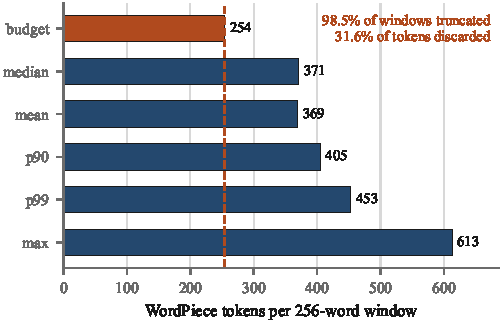
\includegraphics[width=\columnwidth]{figures/12_token_budget.pdf}
\caption{Window length in WordPiece tokens against the $254$-token
content budget, over $14{,}558$ windows from $356$ screenplays. The
window is specified in words; truncation happens in tokens.}
\label{fig:tokens}
\end{figure}

\subsection{Lexical control}

The lexical control is TF-IDF over unigrams and bigrams, capped at
$8{,}000$ features, with English stop words removed, minimum document
frequency $3$, maximum document frequency $0.85$, and sublinear term
frequency $1 + \log \mathrm{tf}$. It is fitted on aggressively normalised
text --- lowercased, stage directions and speaker cues stripped,
punctuation reduced --- and fed to the same gradient-boosted regressor as
the semantic arm. This pairing is deliberate: SBERT and TF-IDF differ in
representation and in nothing else, so their gap is attributable to
semantics rather than to the learner.

\subsection{Learners}

The regressor throughout is gradient-boosted trees with $500$ rounds,
learning rate $0.05$, maximum depth $6$, histogram splitting, and early
stopping after $20$ rounds without validation improvement; predictions
are clipped to $[1, 10]$. Two linear probes provide reference points:
ordinary least squares on the three metadata columns, and ridge
regression ($\alpha = 1.5$) on standardised embeddings. A
constant-mean predictor anchors the bottom.

\subsection{Partition protocols}
\label{sec:splits}

Let $\mathcal{I} = \{1, \dots, n\}$ index the analysis corpus,
$n = 5{,}164$.

\hlt{P1, random.} A shuffled $K$-fold partition, $K = 5$: disjoint
$F_1, \dots, F_K$ with $\bigcup_k F_k = \mathcal{I}$, assignment
independent of every record attribute.

\hlt{P2, grouped.} Let $\gamma: \mathcal{I} \to \mathcal{G}$ map each
record to its title family, $|\mathcal{G}| = 4{,}979$.
\textsc{GroupKFold} constructs disjoint folds subject to the group
constraint
\begin{equation}
\label{eq:group}
\forall g \in \mathcal{G}\;\; \exists!\, k \in \{1,\dots,K\}:\;
\gamma^{-1}(g) \subseteq F_k ,
\end{equation}
so no family is split across the boundary, while the fold sizes
$|F_k|$ are balanced as far as \eqref{eq:group} permits. Because
$4{,}979$ families cover $5{,}164$ records, the constraint is nearly
free: realised fold sizes are $1{,}032$--$1{,}033$, identical to P1.

\hlt{P3, chronological.} With $\mathrm{yr}(i)$ the release year,
\begin{align}
\mathcal{T}_{\text{test}} &= \{\, i : 2020 \le \mathrm{yr}(i) \le 2025 \,\},\\
\mathcal{T}_{\text{val}}  &= \{\, i : c \le \mathrm{yr}(i) \le 2019 \,\},\\
\mathcal{T}_{\text{train}}&= \{\, i : \mathrm{yr}(i) < c \,\},
\end{align}
where $c$ is the $85$th percentile of the pre-2020 year distribution,
here $c = 2016$. Early stopping is thereby decided on films that are
themselves in the future relative to the training set, so no
forward-looking information enters through model selection. The realised
sizes are $3{,}918$ / $731$ / $515$.

A partition's leakage can be measured directly. Define the family-overlap
rate of a test fold as the share of its records whose family also occurs
in the corresponding training pool,
\begin{equation}
\lambda(F_k) = \frac{1}{|F_k|}
\bigl|\{\, i \in F_k : \gamma(i) \in \gamma(\mathcal{I} \setminus F_k) \,\}\bigr| .
\end{equation}
Averaged over folds, $\lambda = 5.50\%$ under P1 and, by construction,
$\lambda = 0$ under P2. The chronological holdout sits at
$\lambda = 6.41\%$ --- a sequel released in 2021 may well have a parent
film in the training years, and eliminating that would require dropping
whole franchises rather than merely reassigning them.

\subsection{Inference}

Point estimates carry percentile bootstrap intervals from $B = 1000$
resamples of the test set. Model comparison is paired and
distribution-free. For predictions $\hat{y}^{A}$, $\hat{y}^{B}$ on a
common test set, form per-record absolute errors
$e^{A}_i = |\hat{y}^{A}_i - y_i|$ and $e^{B}_i$ likewise, take
$d_i = e^{A}_i - e^{B}_i$, discard the $n_0$ exact ties, rank the
remaining $|d_i|$, and accumulate
\begin{equation}
R^{+} = \!\!\sum_{i:\, d_i > 0}\!\! \mathrm{rank}(|d_i|),
\qquad
R^{-} = \!\!\sum_{i:\, d_i < 0}\!\! \mathrm{rank}(|d_i|) ,
\end{equation}
with test statistic $W = \min(R^{+}, R^{-})$. The signed-rank test is
non-parametric and has no degrees-of-freedom parameter; the reporting
quantities are the number of pairs $n$, the number of non-tied pairs
$n - n_0$, the statistic $W$, and the matched-pairs rank-biserial effect
size
\begin{equation}
r \;=\; \frac{R^{+} - R^{-}}{R^{+} + R^{-}} \;\in\; [-1, 1] ,
\end{equation}
which we report alongside $p$ so that a small effect at large $n$ is not
mistaken for a large one. Differences in mean absolute error carry their
own paired bootstrap intervals.

% =====================================================================
\section{Experimental Results}
\label{sec:results}

\subsection{The cost of a stricter partition}

Table~\ref{tab:grouped} isolates the cost of the group constraint;
Table~\ref{tab:temporal} isolates the cost of the temporal one. Five
systems, one corpus, one learner configuration throughout.

\begin{table*}[t]
\caption{Grouped five-fold results. P1 shuffles records; P2 enforces the
title-family constraint \eqref{eq:group}. Pooled out-of-fold point
estimates with $95\%$ percentile bootstrap intervals over $5{,}164$
records. $\Delta R^{2}$ is the explained variance lost to the constraint,
i.e.\ the share of P1 skill that franchise overlap was supplying.}
\label{tab:grouped}
\centering
\small
\begin{tabular}{lccc@{\hskip 18pt}ccc@{\hskip 18pt}c}
\toprule
& \multicolumn{3}{c}{\textbf{P1 random $k$-fold} ($\lambda = 5.50\%$)}
& \multicolumn{3}{c}{\textbf{P2 grouped by family} ($\lambda = 0\%$)} & \\
\cmidrule(lr){2-4}\cmidrule(lr){5-7}
\textbf{System} & RMSE & MAE & $R^{2}$ & RMSE & MAE & $R^{2}$ & $\Delta R^{2}$ \\
\midrule
Constant mean          & 1.4373 & 1.1761 & $-0.0000$ & 1.4375 & 1.1765 & $-0.0004$ & $-0.0004$ \\
Metadata OLS           & 1.1237 & 0.8701 & 0.3888 & 1.1236 & 0.8695 & 0.3889 & $+0.0001$ \\
SBERT ridge            & 1.1122 & 0.8618 & 0.4012 & 1.1238 & 0.8742 & 0.3887 & $-0.0125$ \\
SBERT + XGBoost        & 1.0907 & 0.8355 & 0.4241 & 1.1026 & 0.8445 & 0.4114 & $-0.0127$ \\
SBERT + meta + XGBoost & \textbf{0.9652} & \textbf{0.7276} & \textbf{0.5490}
                       & \textbf{0.9791} & \textbf{0.7309} & \textbf{0.5359} & $-0.0131$ \\
\addlinespace[2pt]
\multicolumn{8}{l}{\footnotesize Best system: P1 $R^{2}\in[0.5298,0.5671]$,
P2 $R^{2}\in[0.5162,0.5537]$. Every arm that reads text loses $R^{2}$;
the metadata-only probe does not.}\\
\bottomrule
\end{tabular}
\end{table*}

\begin{table}[t]
\caption{Temporal holdout. Fit on films released up to $2015$, early
stopping on $2016$--$2019$, tested on the $515$ films released
$2020$--$2025$. Point estimates with $95\%$ percentile bootstrap
intervals.}
\label{tab:temporal}
\centering
\small
\begin{tabular}{lccc}
\toprule
\textbf{System} & RMSE & MAE & $R^{2}$ \\
\midrule
Constant mean   & 1.2230 & 0.9762 & $-0.0947$ \\
Metadata OLS    & 1.0794 & 0.8384 & 0.1473 \\
SBERT ridge     & 1.0719 & 0.8417 & 0.1591 \\
SBERT + XGBoost & 1.0007 & 0.7469 & 0.2671 \\
SBERT + meta + XGBoost & \textbf{0.9717} & \textbf{0.7232} & \textbf{0.3089} \\
\addlinespace[2pt]
\multicolumn{4}{l}{\footnotesize Best system $R^{2}\in[0.1985,0.4038]$;
$n = 3{,}918 / 731 / 515$; $\lambda = 6.41\%$.}\\
\multicolumn{4}{l}{\footnotesize Target: train $6.0119 \pm 1.4619$,
holdout $5.7546 \pm 1.1701$.}\\
\bottomrule
\end{tabular}
\end{table}

Fig.~\ref{fig:protocols} plots all three protocols with their intervals.
Grouping costs little. The best system moves from $R^{2} = 0.5490$ to
$0.5359$, a drop of $0.0131$, and the two bootstrap intervals overlap
substantially. That is the expected result for a corpus in which
$4{,}979$ families cover $5{,}164$ records: only $164$ families have more
than one member and the largest has four, so the group constraint
reassigns few records. The interesting part is that the effect is
consistently negative across every system that reads text --- SBERT ridge
loses $0.0125$ $R^{2}$, SBERT+XGBoost loses $0.0127$ --- while the
metadata-only probe is unmoved ($0.3888 \to 0.3889$). Franchise leakage
is a \emph{textual} channel, and a metadata model cannot exploit it
because it never sees the words.

Chronology costs a great deal. The same best system falls to
$R^{2} = 0.3089$, and the interval $[0.1985, 0.4038]$ no longer overlaps
either in-corpus estimate. Two mechanisms are separable in the table. The
constant-mean predictor goes from $R^{2} \approx 0$ to $-0.0947$, which
is a pure distribution-shift effect: the training mean ($6.11$) is
simply wrong for the holdout ($5.75$). And the metadata probe collapses
hardest of all, from $0.3889$ to $0.1473$, losing $62\%$ of its
explanatory power, while the text-only SBERT model loses $35\%$
($0.4114 \to 0.2671$). The representation that generalises worst across
time is the one that was never about the film.

\begin{figure*}[t]
\centering
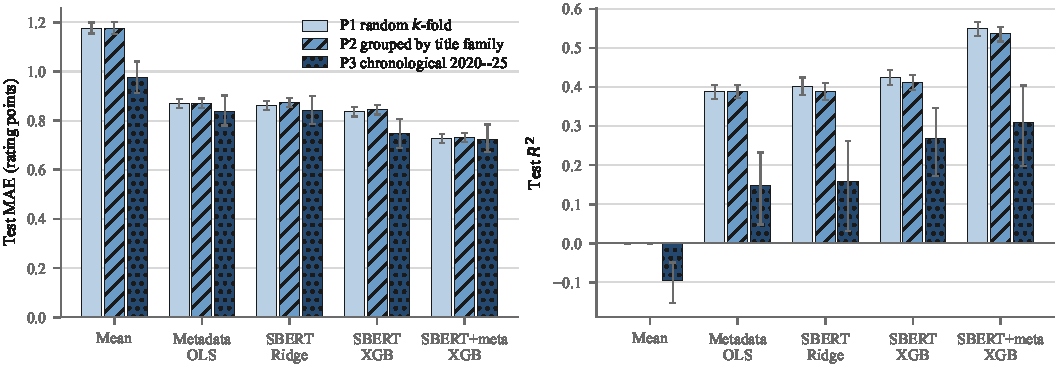
\includegraphics[width=\textwidth]{figures/11_protocols.pdf}
\caption{Test error and explained variance under the three protocols.
Bars are point estimates, whiskers $95\%$ bootstrap intervals. Every
system degrades from P1 to P3; the metadata probe degrades most.}
\label{fig:protocols}
\end{figure*}

\subsection{Paired comparisons}

Table~\ref{tab:paired} reports every baseline against the best system on
matched records.

\begin{table}[t]
\caption{Paired comparison against SBERT + metadata + XGBoost.
$\Delta\mathrm{MAE}$ is positive when the reference system has lower
error. $p$ from the two-sided Wilcoxon signed-rank test.}
\label{tab:paired}
\centering
\small
\begin{tabular}{llrrr}
\toprule
\textbf{Prot.} & \textbf{Baseline} & $\Delta\mathrm{MAE}$ & \textbf{95\% CI} & $p$ \\
\midrule
\multirow{4}{*}{P1}
 & Constant mean   & $+0.4485$ & $[+0.427, +0.471]$ & $2.2\!\times\!10^{-281}$ \\
 & Metadata OLS    & $+0.1425$ & $[+0.129, +0.157]$ & $1.8\!\times\!10^{-73}$ \\
 & SBERT ridge     & $+0.1342$ & $[+0.116, +0.150]$ & $7.0\!\times\!10^{-55}$ \\
 & SBERT + XGB     & $+0.1079$ & $[+0.093, +0.122]$ & $4.7\!\times\!10^{-46}$ \\
\addlinespace[2pt]
\multirow{4}{*}{P2}
 & Constant mean   & $+0.4456$ & $[+0.424, +0.466]$ & $2.9\!\times\!10^{-280}$ \\
 & Metadata OLS    & $+0.1386$ & $[+0.124, +0.152]$ & $2.8\!\times\!10^{-73}$ \\
 & SBERT ridge     & $+0.1433$ & $[+0.127, +0.159]$ & $2.5\!\times\!10^{-61}$ \\
 & SBERT + XGB     & $+0.1136$ & $[+0.100, +0.127]$ & $2.1\!\times\!10^{-50}$ \\
\addlinespace[2pt]
\multirow{4}{*}{P3}
 & Constant mean   & $+0.2530$ & $[+0.195, +0.313]$ & $5.7\!\times\!10^{-15}$ \\
 & Metadata OLS    & $+0.1152$ & $[+0.063, +0.166]$ & $2.0\!\times\!10^{-4}$ \\
 & SBERT ridge     & $+0.1185$ & $[+0.064, +0.176]$ & $1.3\!\times\!10^{-4}$ \\
 & SBERT + XGB     & $+0.0236$ & $[-0.020, +0.074]$ & $0.273$ \\
\bottomrule
\end{tabular}
\end{table}

The final row is the one that changes the story. Under P1 and P2, adding
the three metadata columns to the embedding buys a highly significant
$0.108$--$0.114$ rating points of mean absolute error. Under P3 the same
addition buys $0.0236$ points, with an interval straddling zero and
$p = 0.273$; the full statistics are $W = 62{,}734$ over $n = 515$ pairs
with no ties, rank-biserial $r = +0.056$. An effect size of $0.056$ is
negligible by any convention. The metadata block, worth two orders of
magnitude in $p$-value under a random split, is not measurably useful
when the test films are genuinely unseen.

\subsection{The lexical and structural arms}

The lexical control and the structural-feature model can be evaluated
only under the random protocol on this corpus, because reconstructing
either representation requires the raw script text (Section
\ref{sec:hashscope}). Table~\ref{tab:legacy} reproduces those figures
from the archived runs for completeness.

\begin{table}[t]
\caption{Random-protocol results for the arms that require raw text
($5$-fold CV, mean $\pm$ s.d.; archived runs over $5{,}195$ records).
These are \emph{not} comparable to Tables~\ref{tab:grouped}--\ref{tab:temporal}.}
\label{tab:legacy}
\centering
\small
\begin{tabular}{lccc}
\toprule
\textbf{System} & RMSE & MAE & $R^{2}$ \\
\midrule
\multicolumn{4}{l}{\emph{Representation arms ($5$-fold CV)}}\\
Structural OLS (16 feats.\ + meta) & $1.076 \pm 0.040$ & $0.833 \pm 0.031$ & $0.440 \pm 0.007$ \\
TF-IDF + XGBoost                    & $1.083 \pm 0.034$ & $0.819 \pm 0.022$ & $0.433 \pm 0.014$ \\
SBERT + XGBoost (weighted)          & $1.000 \pm 0.027$ & $0.768 \pm 0.024$ & $0.516 \pm 0.026$ \\
SBERT + XGBoost (unweighted)        & $0.958 \pm 0.033$ & $0.720 \pm 0.027$ & $0.556 \pm 0.009$ \\
\addlinespace[3pt]
\multicolumn{4}{l}{\emph{Ensembling and tuning}}\\
SBERT + XGBoost (stack base)        & $0.956 \pm 0.034$ & $0.719 \pm 0.028$ & $0.558 \pm 0.013$ \\
Ridge stack over 4 base models      & $0.935 \pm 0.032$ & $0.706 \pm 0.028$ & $0.577 \pm 0.010$ \\
SBERT + XGBoost, 100-trial TPE$^{\dagger}$ & $0.966$ & $0.714$ & $0.581$ \\
\addlinespace[2pt]
\multicolumn{4}{l}{\footnotesize $^{\dagger}$single $80/20$ split with
bootstrap intervals, not $5$-fold CV.}\\
\bottomrule
\end{tabular}
\end{table}

Three points survive the caveat. The lexical and structural arms land
within $0.007$ $R^{2}$ of each other --- $8{,}000$ TF-IDF weights buy
almost exactly what sixteen hand-counted statistics buy, which says
something unflattering about both. The semantic arm beats the lexical one
by $\Delta\mathrm{MAE} = 0.0514$ $[0.034, 0.067]$,
$p = 2.6\times10^{-5}$, a real but modest margin. And inverse-frequency
sample weighting, applied in the original pipeline to compensate for the
rating imbalance, \emph{hurts}: removing it improves MAE by $0.0482$
$[0.039, 0.057]$ at $p = 2.5\times10^{-26}$. Reweighting a regression
target by frequency bucket optimises a criterion nobody reported.

The lower block of Table~\ref{tab:legacy} covers two further archived
experiments in the same random-protocol regime. A ridge meta-regressor
stacked over four base models --- metadata OLS, structural OLS,
TF-IDF+XGBoost, SBERT+XGBoost --- with inner five-fold out-of-fold
meta-features improves on its own strongest base by
$\Delta\mathrm{MAE} = 0.0134$ $[0.008, 0.019]$,
$p = 4.2\times10^{-6}$. A $100$-trial TPE search over the boosting head
reaches test $R^{2} = 0.5811$ $[0.5471, 0.6182]$. Both gains are real and
both are small next to the $0.240$ $R^{2}$ that separates the random and
chronological protocols in Tables~\ref{tab:grouped} and~\ref{tab:temporal}.
Ensembling and tuning move the third decimal; the split moves the first.

Whether the lexical arm would overtake the semantic arm under a
chronological split is exactly the question this corpus cannot currently
answer, and we decline to guess. The prior in either direction is weak:
TF-IDF vocabulary is tied to the training era and might transfer worse,
while frozen sentence embeddings encode general semantics and might
transfer better. Section~\ref{sec:limits} states the experiment we would
run.

\subsection{Temporal shift in detail}

The holdout target is compressed relative to the training pool: standard
deviation falls from $1.4619$ (records up to 2019) to $1.1701$
(2020--2025), while the mean falls from $6.0119$ to $5.7546$. Part of the
$R^{2}$ collapse is therefore arithmetic --- the same absolute error
against a narrower target yields a smaller $R^{2}$ --- and part is
genuine degradation. Mean absolute error separates them: it is $0.7276$
under P1 and $0.7232$ under P3, statistically indistinguishable. The
model's typical error in rating points does not grow at all when it
predicts the future. What collapses is how much of the (now narrower)
variance it can order.

Per-year behaviour (Fig.~\ref{fig:temporal}, left) shows mild, drifting
bias rather than a break: predictions run $+0.27$ high in 2021 and
$+0.23$ high in 2022, then swing to $-0.24$ low in 2025, with per-year
MAE between $0.641$ and $0.799$. Regressing prediction on truth over the
holdout gives slope $0.4634$ $(\mathrm{s.e.}\ 0.0278)$ and intercept
$3.1745$, against an ideal slope of $1$; the predicted standard deviation
is $0.783$ of the observed one. Fig.~\ref{fig:temporal} (right) shows the
resulting fan. The system is heavily shrunk toward the centre --- it
identifies which films are above or below average and declines to commit
to how far.

\begin{figure*}[t]
\centering
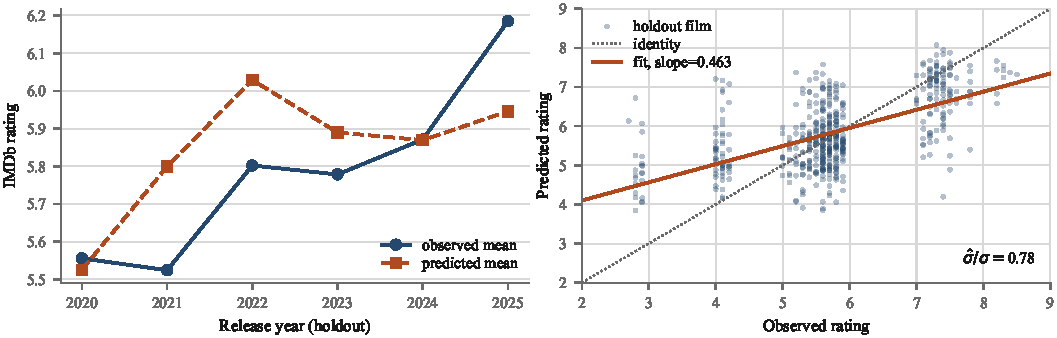
\includegraphics[width=\textwidth]{figures/13_temporal.pdf}
\caption{Chronological holdout. Left: observed and predicted mean rating
by release year ($n = 84, 90, 94, 111, 90, 46$ for 2020--2025). Right:
per-film predictions against truth, with the fitted calibration line;
slope $0.463$ against an ideal of $1$.}
\label{fig:temporal}
\end{figure*}

\subsection{Variable definitions}

Table~\ref{tab:vardef} is the reference for every non-embedding
predictor. Definitions are transcribed from the extraction code rather
than restated informally, because two of them turn out to measure
transcription convention rather than screenwriting
(Section~\ref{sec:method}) and the distinction is only visible in the
operational definition. Gain shares are from the shipped model and sum
with the $384$ embedding dimensions to $100\%$.

\begin{table*}[t]
\caption{The nineteen numeric predictors: operational definition, scale
on the fitted corpus, and share of total split gain. $W$ is the word
sequence, $L$ the line sequence, $S$ the sentence sequence obtained by
splitting on $[.!?]^{+}$, all computed on the raw file.}
\label{tab:vardef}
\centering
\small
\begin{tabular}{llrr}
\toprule
\textbf{Variable} & \textbf{Definition} & \textbf{Mean $\pm$ s.d.} & \textbf{Gain (\%)} \\
\midrule
\multicolumn{4}{l}{\emph{Size and structure}}\\
\texttt{char\_count}           & $|\,\text{raw text}\,|$ in characters                        & $56{,}341 \pm 45{,}050$ & 2.41 \\
\texttt{word\_count}           & $|W|$, whitespace split                                      & $9{,}916 \pm 7{,}003$   & 1.56 \\
\texttt{line\_count}           & $|L|$, newline split                                         & $2{,}483 \pm 1{,}826$   & 0.75 \\
\texttt{sentence\_count}       & $|S|$                                                        & $1{,}610 \pm 873$       & 0.66 \\
\texttt{scene\_count}          & count of case-insensitive \texttt{INT.}/\texttt{EXT.} matches & $19.0 \pm 54.5$        & 0.47 \\
\texttt{words\_per\_scene}     & $|W| / \max(\texttt{scene\_count}, 1)$; inverse tempo         & $6{,}700 \pm 4{,}598$   & 0.65 \\
\addlinespace[3pt]
\multicolumn{4}{l}{\emph{Lexical sophistication}}\\
\texttt{avg\_word\_length}     & $\frac{1}{|W|}\sum_{w \in W} |w|$                            & $4.31 \pm 0.23$         & 0.26 \\
\texttt{unique\_word\_ratio}   & $|\{W\}| / |W|$, type--token ratio                           & $0.298 \pm 0.057$       & 0.16 \\
\texttt{long\_word\_ratio}     & $|\{w \in W : |w| \ge 8\}| / |W|$                            & $0.089 \pm 0.026$       & 0.09 \\
\addlinespace[3pt]
\multicolumn{4}{l}{\emph{Sentence geometry}}\\
\texttt{avg\_sentence\_length} & mean of $|s|$ in words, $s \in S$                            & $6.74 \pm 19.95$        & 0.17 \\
\texttt{sentence\_length\_std} & population s.d.\ of $|s|$, $s \in S$                         & $6.27 \pm 16.90$        & 0.21 \\
\addlinespace[3pt]
\multicolumn{4}{l}{\emph{Dialogue (format-sensitive; see \S\ref{sec:method})}}\\
\texttt{dialogue\_density}     & ALL-CAPS speaker-cue lines $/\,|L|$                          & $0.0087 \pm 0.0361$     & 0.09 \\
\texttt{unique\_characters}    & distinct speaker-cue names                                   & $3.41 \pm 10.77$        & 0.05 \\
\addlinespace[3pt]
\multicolumn{4}{l}{\emph{Affect and direction proxies}}\\
\texttt{exclamation\_ratio}    & $100 \cdot \#\{\texttt{!}\} / |W|$                           & $1.73 \pm 1.61$         & 0.22 \\
\texttt{question\_ratio}       & $100 \cdot \#\{\texttt{?}\} / |W|$                           & $2.95 \pm 1.11$         & 0.13 \\
\texttt{action\_density}       & $100 \cdot (\#\text{bracketed} + \#\text{parenthesised}) / |W|$ & $0.85 \pm 1.85$      & 0.10 \\
\midrule
\multicolumn{2}{l}{\textbf{Structural subtotal (16 variables)}}    &                    & \textbf{7.98} \\
\midrule
\multicolumn{4}{l}{\emph{Metadata (not derived from the script)}}\\
\texttt{movie\_length}         & runtime in minutes, median-imputed                           & $104.2 \pm 20.0$        & 25.50 \\
\texttt{year}                  & release year                                                 & $1999.9 \pm 33.4$       & 11.01 \\
\texttt{decade\_encoded}       & ordinal label encoding of the decade string, $14$ levels      & $10.24 \pm 2.50$        & 0.06 \\
\midrule
\multicolumn{2}{l}{\textbf{Metadata subtotal (3 variables)}}       &                    & \textbf{36.57} \\
\multicolumn{2}{l}{\textbf{SBERT subtotal (384 dimensions)}}       &                    & \textbf{55.45} \\
\bottomrule
\end{tabular}
\end{table*}

% =====================================================================
\section{What the Features Are Doing}
\label{sec:xai}

\subsection{In-sample gain is not out-of-sample use}

Fig.~\ref{fig:importance}(a) splits the shipped model's total split gain
across the three feature blocks. The $384$ embedding dimensions take
$55.5\%$, the three metadata columns take $36.6\%$, and the sixteen
structural statistics take $8.0\%$. Per dimension the picture inverts:
the single largest embedding dimension contributes $1.68\%$ and the mean
dimension $0.14\%$, whereas \texttt{movie\_length} alone contributes
$25.50\%$ and \texttt{year} $11.01\%$. One tabular column outweighs all
sixteen structural statistics by a factor of three.

Within the structural block the ordering is almost purely a size
ordering. Character count ($2.41\%$), word count ($1.56\%$), line count
($0.75\%$), and sentence count ($0.66\%$) occupy the top four positions;
they are four measurements of the same latent quantity, script length,
which is itself a proxy for runtime. The tempo measure
\texttt{words\_per\_scene} follows at $0.65\%$. At the bottom sit the
features that were supposed to capture craft: \texttt{action\_density}
($0.10\%$, rank $246$ of $403$), \texttt{dialogue\_density} ($0.09\%$,
rank $275$), \texttt{long\_word\_ratio} ($0.09\%$, rank $285$), and
\texttt{unique\_characters} ($0.05\%$, rank $377$). The last two are the
degenerate features flagged in Section~\ref{sec:method}; the model
correctly declines to use them.

\begin{figure*}[t]
\centering
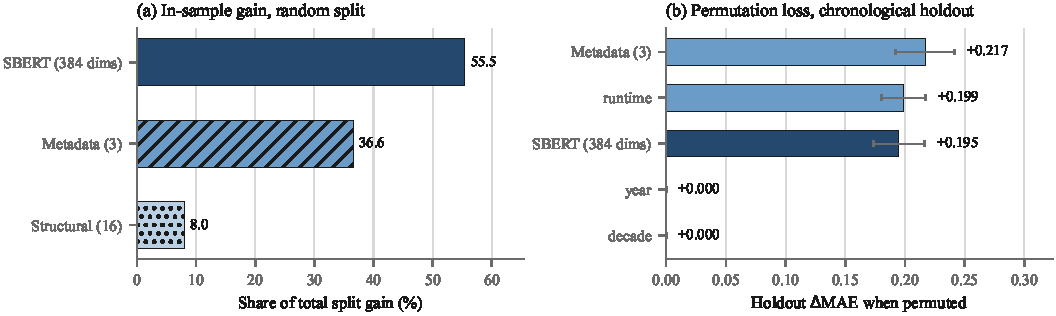
\includegraphics[width=\textwidth]{figures/14_importance.pdf}
\caption{(a) Share of total split gain by feature block in the shipped
model. (b) Increase in holdout MAE when a block is permuted, over $20$
repetitions ($\pm$ s.d.). Year and decade have no measurable use once the
test years lie outside the training range.}
\label{fig:importance}
\end{figure*}

\subsection{Block permutation on the temporal holdout}

Gain is computed on training splits and therefore inherits every
in-sample advantage. Permutation on the holdout does not. We shuffle each
feature block across the $515$ holdout films, re-predict, and record the
increase in MAE over $20$ repetitions; the baseline is
$\mathrm{MAE} = 0.7232$. Fig.~\ref{fig:importance}(b) reports the result,
and it is stark:
\begin{itemize}
\item permuting all three metadata columns: $+0.2168 \pm 0.0250$;
\item permuting \texttt{movie\_length} alone: $+0.1988 \pm 0.0185$;
\item permuting the entire $384$-dimensional embedding:
      $+0.1950 \pm 0.0217$;
\item permuting \texttt{year}: $+0.0000 \pm 0.0000$;
\item permuting \texttt{decade\_encoded}: $+0.0000 \pm 0.0000$.
\end{itemize}

The two zeros are not rounding. Every holdout film was released in
2020--2025, and the model was fitted on films up to 2015, so every
holdout value of \texttt{year} lies beyond the largest training split
threshold. A tree ensemble routes all of them down the same branch;
shuffling values that already share a leaf changes nothing. The feature
carrying $11\%$ of in-sample gain becomes a constant at deployment.
\texttt{decade\_encoded} is worse still --- $0.06\%$ of gain in-sample,
corrupt levels in its vocabulary, and no effect out of sample.

Runtime is the opposite case. It transfers cleanly, because a
$130$-minute film in 2023 occupies the same region of feature space as a
$130$-minute film in 1994, and it alone reproduces the predictive value
of the entire semantic block. The honest summary of the temporal result
is that the model has two working channels: how long the film is, and
what the screenplay is broadly about. The calendar is not one of them.

\subsection{Why mean pooling limits the semantic channel}

The embedding block earns $+0.195$ MAE under permutation, so it carries
real signal, but its per-dimension gain is flat --- no dimension exceeds
$1.7\%$ and none is unused. That is the signature of a diffuse
representation, and Eq.~\eqref{eq:norm} explains it. Averaging $36$
median unit-norm window embeddings drives the document vector toward the
centroid of the corpus, damping precisely the localised evidence --- a
sharp scene, an unusual register --- that a human reader would use to
judge a script. Combined with the $31.6\%$ of tokens that truncation
removes before pooling begins, the semantic channel is operating on a
heavily smoothed, partially observed view of the screenplay. That it
still contributes as much as it does is the more surprising half of the
result.

% =====================================================================
\section{Threats to Validity and Limitations}
\label{sec:limits}

\hlt{The content-digest audit is verified on a subset.} As stated in
Section~\ref{sec:hashscope}, SHA-256 deduplication was executed over the
$356$ script files distributed with the code and returned zero duplicate
groups. The remaining $4{,}848$ files are not redistributed, so the
corpus-wide exact-duplicate rate is unmeasured. The metadata identity
keys covering all $5{,}204$ records found no duplicate identifiers and no
duplicate title$\times$year pairs, which bounds the plausible residual
duplication, but does not eliminate the possibility of two distinct
films sharing a byte-identical file through a scraping error. We report
this rather than assert a number we did not compute.

\hlt{Two arms are missing from the strict protocols.} TF-IDF and the
sixteen structural statistics require raw text and could therefore be
evaluated only under P1. The paper's temporal comparison is consequently
between semantic embeddings, metadata, and their combination. Restoring
the corpus makes the full three-way comparison a single re-run of the
released scripts, and we regard that as the first experiment any
extension should perform.

\hlt{Selection effects in IMSDb are severe and not correctable.}
Contributors upload what they value, so canonical and acclaimed films are
over-represented among older titles while recent years sample more
broadly. The corpus-wide mean rating falls monotonically from $7.87$ in
the 1920s to $5.48$ in the 2010s, which is a statement about who uploads
what, not about film quality. Any model reading \texttt{year} learns this
curation artifact, and P3 is the protocol that refuses to reward it.
Generalisation claims extend to films resembling IMSDb's selection, not
to an arbitrary IMDb title.

\hlt{Temporal target compression confounds $R^{2}$.} The holdout's
rating standard deviation is $0.80\times$ the training pool's. Because
$R^{2}$ is normalised by target variance, part of the $0.536 \to 0.309$
drop is definitional. We report MAE alongside for this reason, and MAE is
flat across protocols. Readers should treat the $R^{2}$ collapse as a
statement about \emph{rank-ordering power on recent films}, not about
absolute error growth.

\hlt{The holdout is one window.} A single 2020--2025 test period of $515$
films cannot separate a general temporal-decay law from the particulars of
those six years, which include a pandemic-disrupted release calendar and
a shift toward streaming premieres. Rolling-origin evaluation over
several cut years would estimate the decay rate; we report one cut.

\hlt{The strongest transferring feature is unavailable at deployment.}
Runtime dominates the temporal holdout, matching the entire embedding
block under permutation. A screenplay-stage predictor does not know the
runtime, because the film has not been cut --- or shot. The repository's
own inference path concedes the point: when metadata is not supplied it
substitutes constants, defaulting \texttt{movie\_length} to $120$
minutes, \texttt{year} to $2020$, and \texttt{decade\_encoded} to $0$.
Under those defaults the deployed system is closer to our SBERT-only
row ($R^{2} = 0.267$ on the holdout) than to the headline. Page count is
a legitimate pre-production proxy for runtime and is recoverable from the
script; we did not evaluate it, and it is the obvious substitution to
test next.

\hlt{Observational ceiling.} An IMDb rating aggregates audience response
to a finished film --- casting, direction, editing, marketing, release
timing --- of which the screenplay is one input. No script-only model can
exceed the share of rating variance attributable to the script, and that
ceiling is unknown. The results here should be read as a lower bound on
achievable skill and, more usefully, as a measurement of how much of the
apparent skill was an artifact of the split.

\hlt{Single encoder, single pooling.} We audit mean-pooled
\texttt{all-MiniLM-L6-v2}. Larger encoders, learned pooling, and
token-aligned windows are all plausible improvements, and none is
evaluated here; the point of the paper is the protocol, and holding the
representation fixed is what makes the protocol comparison clean.

% =====================================================================
\section{Conclusion}

We audited a screenplay-to-rating pipeline instead of extending it. The
corpus turned out to be clean at the record level --- $5{,}204$ distinct
identifiers, no repeated title$\times$year pair --- but to carry $164$
multi-member title families, four corrupt release years, and a corrupt
ordinal decade vocabulary that reaches the feature matrix intact. The
chunking configuration turned out to discard $31.60\%$ of WordPiece
tokens without warning, because the window is measured in words and the
budget is measured in tokens. And the headline metric turned out to
depend on the partition far more than on the model: $R^{2} = 0.549$ under
random folds, $0.536$ once franchises are kept together, $0.309$ when the
test films are drawn from years the model never saw.

The block-permutation analysis identifies the mechanism. Release year
supplies $11\%$ of in-sample split gain and exactly zero out-of-sample
utility, because every holdout year falls beyond the training range and a
tree ensemble cannot extrapolate past its last split point. Runtime
transfers; semantics transfer; the calendar does not. For anyone building
a screenplay-stage predictor, the operational recommendations are
narrow and concrete: group by title family, hold out by release year,
report MAE next to $R^{2}$ when the target distribution shifts, align the
chunk to the tokeniser rather than to whitespace, and store an immutable
record key beside every cached representation.

% =====================================================================
\section*{Reproducibility}

The audit, alignment-recovery, evaluation, and figure code are released
with the paper (\texttt{audit\_corpus.py}, \texttt{recover\_alignment.py},
\texttt{audit\_tokens.py}, \texttt{leakage\_eval.py},
\texttt{analysis\_xai.py}, \texttt{make\_paper\_figures.py}). Every
number in Tables~\ref{tab:audit}--\ref{tab:legacy} and every figure is
regenerated from the committed JSON artifacts in \texttt{results/}. The
random seed is $42$ throughout; bootstrap resampling uses $1000$ draws.

% =====================================================================
\begin{thebibliography}{99}

\bibitem{ref1}
I.~Beltagy, M.~E.~Peters, and A.~Cohan, ``Longformer: The long-document
transformer,'' \emph{arXiv:2004.05150}, 2020.

\bibitem{ref2}
N.~Reimers and I.~Gurevych, ``Sentence-BERT: Sentence embeddings using
Siamese BERT-networks,'' in \emph{Proc.\ EMNLP}, 2019.

\bibitem{ref3}
J.~Eliashberg, S.~K.~Hui, and Z.~J.~Zhang, ``Assessing box office
performance using movie scripts: A kernel-based approach,''
\emph{IEEE Trans.\ Knowl.\ Data Eng.}, vol.~26, no.~11, 2014.

\bibitem{ref4}
S.~D.~Hunter, S.~Smith, and S.~Singh, ``Predicting box office from the
screenplay: A text analytical approach,'' West East Institute, 2016.

\bibitem{ref5}
A.~J.~Reagan, L.~Mitchell, D.~Kiley, C.~M.~Danforth, and P.~S.~Dodds,
``The emotional arcs of stories are dominated by six basic shapes,''
\emph{EPJ Data Science}, vol.~5, no.~31, 2016.

\bibitem{ref6}
A.~Ramakrishna, V.~R.~Mart{\'i}nez, N.~Malandrakis, K.~Singla, and
S.~Narayanan, ``Linguistic analysis of differences in portrayal of movie
characters,'' in \emph{Proc.\ ACL}, 2017.

\bibitem{ref10}
M.~Shafaei, C.~Smailis, I.~Kakadiaris, and T.~Solorio, ``Age suitability
rating: Predicting MPAA ratings based on movie dialogues,'' in
\emph{Proc.\ LREC}, 2020.

\bibitem{ref11}
Y.~Zhang, M.~Shafaei, and T.~Solorio, ``From none to severe: Predicting
severity in movie scripts,'' in \emph{Findings of EMNLP}, 2021.

\bibitem{ref12}
E.~Chu, D.~Roy, and J.~Glass, ``Audio-visual sentiment analysis for
learning emotional arcs in movies,'' in \emph{Proc.\ ICCV}, 2017.

\bibitem{ref15}
R.~Sharda and D.~Delen, ``Predicting box-office success of motion
pictures with neural networks,'' \emph{Expert Systems with
Applications}, vol.~30, no.~2, 2006.

\bibitem{ref16}
C.~T.~Madongo, Z.~Tang, and J.~Hassan, ``Movie box-office revenue
prediction model by mining deep features from trailers using recurrent
neural networks,'' \emph{J.\ Adv.\ Inf.\ Technol.}, 2024.

\bibitem{ref17}
A.~Bhadrashetty and S.~Patil, ``Movie success and rating prediction
using data mining,'' \emph{J.\ Sci.\ Res.\ Technol.}, 2024.

\bibitem{ref18}
M.~Z.~Naeem, F.~Rustam, A.~Mehmood, I.~Ashraf, and G.~S.~Choi,
``Classification of movie reviews using term frequency-inverse document
frequency and optimized machine learning algorithms,'' \emph{PeerJ
Comput.\ Sci.}, 2022.

\bibitem{ref19}
I.~Chalkidis, X.~Dai, M.~Fergadiotis, P.~Malakasiotis, and D.~Elliott,
``An exploration of hierarchical attention transformers for efficient
long document classification,'' \emph{arXiv:2210.05529}, 2022.

\bibitem{ref21}
S.~Asur and B.~A.~Huberman, ``Predicting the future with social media,''
in \emph{Proc.\ IEEE/WIC/ACM Web Intelligence}, 2010.

\bibitem{ref22}
A.~Oghina, M.~Breuss, M.~Tsagkias, and M.~de~Rijke, ``Predicting IMDb
movie ratings using social media,'' in \emph{Proc.\ ECIR}, 2012.

\bibitem{ref23}
G.~Mishne and N.~Glance, ``Predicting movie sales from blogger
sentiment,'' in \emph{AAAI Spring Symposium}, 2006.

\bibitem{ref24}
M.~Mesty{\'a}n, T.~Yasseri, and J.~Kert{\'e}sz, ``Early prediction of
movie box office success based on Wikipedia activity big data,''
\emph{PLoS ONE}, vol.~8, no.~8, 2013.

\bibitem{ref25}
H.~L.~Vogel, \emph{Entertainment Industry Economics}, 10th ed.
Cambridge, U.K.: Cambridge Univ.\ Press, 2020.

\bibitem{ref26}
W.~R.~Bristi, Z.~Zaman, and N.~Sultana, ``Predicting IMDb rating of
movies by machine learning techniques,'' in \emph{Proc.\ ICCCNT}, 2019.

\bibitem{ref27}
A.~L.~Gomes, M.~Ribeiro, and P.~Quaresma, ``Predicting IMDb rating of TV
series with deep learning: The case of Arrow,''
\emph{arXiv:2211.03388}, 2022.

\bibitem{ref28}
J.~Ramos, A.~Pereira, and L.~Cruz, ``Movie rating prediction using
sentiment features,'' in \emph{Proc.\ SALLD}, 2022.

\bibitem{ref29}
V.~Udandarao, A.~Gupta, and S.~Bhattacharya, ``Movie revenue prediction
using machine learning models,'' \emph{arXiv:2405.11651}, 2024.

\bibitem{ref30}
W.~Xie, Y.~Liu, and H.~Chen, ``Predicting movie success with multi-task
learning: GPT-based sentiment and SIR propagation,''
\emph{arXiv preprint}, 2025.

\bibitem{ref34}
E.~Mohamed, M.~Shafaei, and T.~Solorio, ``A first dataset for film age
appropriateness investigation,'' in \emph{Proc.\ LREC}, 2020.

\bibitem{ref35}
S.~Kar, S.~Maharjan, and T.~Solorio, ``Folksonomication: Predicting tags
for movies from plot synopses using emotion flow encoded neural
network,'' in \emph{Proc.\ COLING}, 2018.

\bibitem{ref38}
M.~C.~Chiu, S.~Lin, and W.~Chen, ``Screenplay quality assessment: Can we
predict who gets nominated?'' Nat.\ Univ.\ Singapore, Tech.\ Rep., 2020.

\bibitem{gorman2019}
K.~Gorman and S.~Bedrick, ``We need to talk about standard splits,'' in
\emph{Proc.\ ACL}, 2019.

\bibitem{sogaard2021}
A.~S{\o}gaard, S.~Ebert, J.~Bastings, and K.~Filippova, ``We need to
talk about random splits,'' in \emph{Proc.\ EACL}, 2021.

\bibitem{lewis2021}
P.~Lewis, P.~Stenetorp, and S.~Riedel, ``Question and answer test-train
overlap in open-domain question answering datasets,'' in \emph{Proc.\
EACL}, 2021.

\bibitem{elangovan2021}
A.~Elangovan, J.~He, and K.~Verspoor, ``Memorization vs.\
generalization: Quantifying data leakage in NLP performance
evaluation,'' in \emph{Proc.\ EACL}, 2021.

\bibitem{kapoor2023}
S.~Kapoor and A.~Narayanan, ``Leakage and the reproducibility crisis in
machine-learning-based science,'' \emph{Patterns}, vol.~4, no.~9, 2023.

\bibitem{lazaridou2021}
A.~Lazaridou \emph{et al.}, ``Mind the gap: Assessing temporal
generalization in neural language models,'' in \emph{Proc.\ NeurIPS},
2021.

\bibitem{bender2018}
E.~M.~Bender and B.~Friedman, ``Data statements for natural language
processing,'' \emph{TACL}, vol.~6, 2018.

\bibitem{dodge2021}
J.~Dodge \emph{et al.}, ``Documenting large webtext corpora: A case
study on the Colossal Clean Crawled Corpus,'' in \emph{Proc.\ EMNLP},
2021.

\end{thebibliography}

\end{document}
